
\documentclass[10pt]{standalone}
\usepackage{tikz}
\usepackage{bm}

\begin{document}
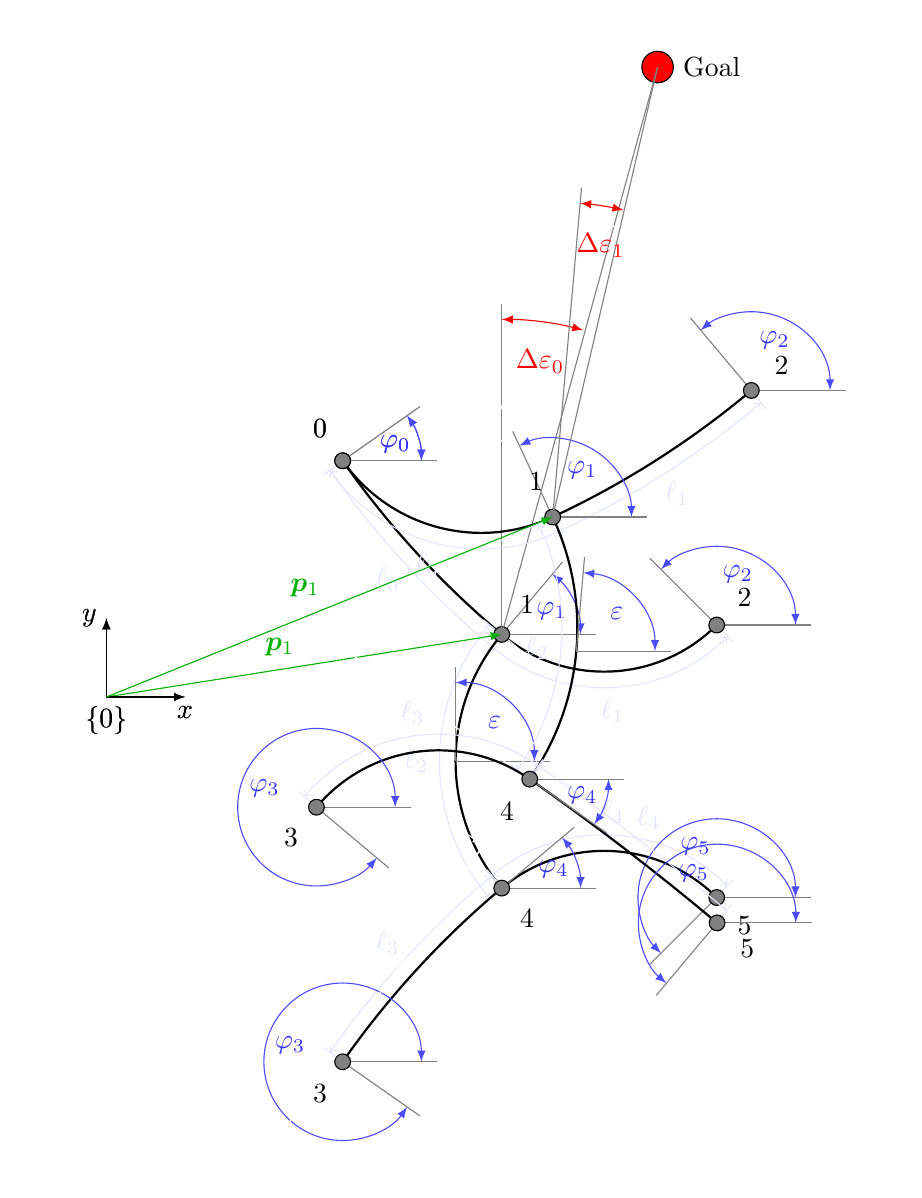
\begin{tikzpicture}[
	part/.style={thick},
	anglearrow/.style={latex-latex, red!0},
	lettering/.style={red!0},
	anglearrow_phi/.style={latex-latex, blue!70},
	lettering_phi/.style={blue!80},
	helpline_phi/.style={gray},
	helpline/.style={white},
	foot/.style={fill=gray},
	distarrow/.style={|<->|, blue!10},
	distlettering/.style={blue!10},
	vec/.style={-latex, green!70!black},
	vechead/.style={green!70!black}
]
\def\pi{3.14159}

\def\rfoot{.1}
\def\rradi{.05}

\def\angledist{1}
\def\fontdist{.7}
\def\distdist{.2}
\def\fontdistdist{.5}

\def\lleg{3}
\def\ltor{3.5}

\newcommand{\drawGecko}[2]{

\pgfmathsetmacro{\gamh}{\gam*.5}
\pgfmathsetmacro{\ci}{\eps-\alpi-\gamh}
\pgfmathsetmacro{\cii}{\ci+\alpi+\beti}
\pgfmathsetmacro{\ciii}{180 + \gam + \ci + \alpi + \alpii}
\pgfmathsetmacro{\civ}{180 + \gam + \ci + \alpi - \betii}



\pgfmathsetmacro{\ri}{\lleg/\alpi*180/\pi}
\pgfmathsetmacro{\rii}{\lleg/\beti*180/\pi}
\pgfmathsetmacro{\rg}{(\ltor/sqrt(\gam*\gam)*180/\pi)*\gam/sqrt(\gam*\gam)}
\pgfmathsetmacro{\riii}{\lleg/\alpii*180/\pi}
\pgfmathsetmacro{\riv}{\lleg/\betii*180/\pi}


%% COS
\path (-2,-2) coordinate(O)node[below]{\{0\}};
\draw[-latex] (O)--++(1,0)node[below]{$x$};
\draw[-latex] (O)--++(0,1)node[left]{$y$};



\path (#1,#2) coordinate(0);
%% F0
\draw[part] (0)arc(180+\ci:180+\ci+\alpi:\ri)coordinate(1);
\draw[helpline] (0)--++(\ci:\ri)coordinate(R0)--(1);
\draw[anglearrow] (R0)++(180+\ci:\angledist)arc(180+\ci:180+\ci+\alpi:\angledist);
\pgfmathsetmacro{\alpih}{\alpi*.5}
\path (R0)++(180+\ci+\alpih:\fontdist) node[lettering]{$\alpha_0$};
\draw[distarrow] (R0)++(180+\ci:\distdist+\ri)arc(180+\ci:180+\ci+\alpi:\distdist+\ri);
\path (R0)++(180+\ci+\alpih:\ri+\fontdistdist) node[distlettering]{$\ell_0$};


%% F1
\draw[part] (1)arc(180+\ci+\alpi:180+\ci+\alpi+\beti:\rii)coordinate(2);
\draw[helpline] (2)--++(\cii:\rii)coordinate(R1)--(1);
\draw[anglearrow] (R1)++(180+\cii:\angledist)arc(180+\cii:180+\cii-\beti:\angledist);
\pgfmathsetmacro{\betih}{\beti*.5}
\path (R1)++(180+\cii-\betih:\fontdist) node[lettering]{$\alpha_1$};
\draw[distarrow] (R1)++(180+\cii-\beti:\distdist+\rii)arc(180+\ci+\alpi:180+\ci+\alpi+\beti:\distdist+\rii);
\path (R1)++(180+\cii-\betih:\rii+\fontdistdist) node[distlettering]{$\ell_1$};


%% T1
\draw[part] (1)arc(90+\ci+\alpi:90+\ci+\alpi+\gam:\rg)coordinate(4);
\draw[helpline] (1)--++(-90+\ci+\alpi:\rg)coordinate(R2)--(4);
\draw[anglearrow] (R2)++(90+\ci+\alpi:\angledist)arc(90+\ci+\alpi:90+\ci+\alpi+\gam:\angledist);
\pgfmathsetmacro{\gamh}{\gam*.5}
\path (R2)++(90+\ci+\alpi+\gamh:\fontdist) node[lettering]{$\alpha_2$};
\draw[distarrow] (R2)++(90+\ci+\alpi:\distdist+\rg)arc(90+\ci+\alpi:90+\ci+\alpi+\gam:\distdist+\rg);
\path (R2)++(90+\ci+\alpi+\gamh:\rg+\fontdistdist) node[distlettering]{$\ell_2$};
\path (R2)++(90+\ci+\alpi+\gamh:\rg)coordinate(M);



%% F2
\draw[part] (4)arc(\gam+\ci+\alpi:\gam+\ci+\alpi+\alpii:\riii)coordinate(3);
\draw[helpline] (3)--++(180+\gam+\ci+\alpi+\alpii:\riii)coordinate(R3)--(4);
\draw[anglearrow] (R3)++(\gam+\ci+\alpi+\alpii:\angledist)arc(\gam+\ci+\alpi+\alpii:\gam+\ci+\alpi:\angledist);
\pgfmathsetmacro{\alpiih}{\alpii*.5}
\path (R3)++(\gam+\ci+\alpi+\alpiih:\fontdist) node[lettering]{$\alpha_3$};
\draw[distarrow] (R3)++(\gam+\ci+\alpi:\distdist+\riii)arc(\gam+\ci+\alpi:\gam+\ci+\alpi+\alpii:\distdist+\riii);
\path (R3)++(\gam+\ci+\alpi+\alpiih:\riii+\fontdistdist) node[distlettering]{$\ell_3$};



%% F3
\draw[part] (4)arc(\gam+\ci+\alpi:\gam+\ci+\alpi-\betii:\riv)coordinate(5);
\draw[helpline] (5)--++(180+\gam+\ci+\alpi-\betii:\riv)coordinate(R4)--(4);
\draw[anglearrow] (R4)++(\gam+\ci+\alpi-\betii:\angledist)arc(\gam+\ci+\alpi-\betii:\gam+\ci+\alpi:\angledist);
\pgfmathsetmacro{\betiih}{\betii*.5}
\path (R4)++(\gam+\ci+\alpi-\betiih:\fontdist) node[lettering]{$\alpha_4$};
\draw[distarrow] (R4)++(\gam+\ci+\alpi:\distdist+\riv)arc(\gam+\ci+\alpi:\gam+\ci+\alpi-\betii:\distdist+\riv);
\path (R4)++(\gam+\ci+\alpi-\betiih:\riv+\fontdistdist) node[distlettering]{$\ell_4$};



%% Constant
\draw[helpline_phi] (0)--++(0:\angledist+.2);
\draw[helpline_phi] (0)--++(\ci:\angledist+.2);
\draw[anglearrow_phi] (0)++(0:\angledist)arc(0:\ci:\angledist);
\pgfmathsetmacro{\cih}{\ci*.5}
\path (0)++(\cih:\fontdist) node[lettering_phi]{$\varphi_0$};

\draw[helpline_phi] (1)--++(0:\angledist+.2);
\draw[helpline_phi] (1)--++(\eps-\gamh:\angledist+.2);
\draw[anglearrow_phi] (1)++(0:\angledist)arc(0:\eps-\gamh:\angledist);
\pgfmathsetmacro{\cih}{(\eps-\gamh)*.5}
\path (1)++(\cih:\fontdist) node[lettering_phi]{$\varphi_1$};


\draw[helpline_phi] (2)--++(0:\angledist+.2);
\draw[helpline_phi] (2)--++(\cii:\angledist+.2);
\draw[anglearrow_phi] (2)++(0:\angledist)arc(0:\cii:\angledist);
\pgfmathsetmacro{\ciih}{\cii*.5}
\path (2)++(\ciih:\fontdist) node[lettering_phi]{$\varphi_2$};

\draw[helpline_phi] (3)--++(0:\angledist+.2);
\draw[helpline_phi] (3)--++(\ciii:\angledist+.2);
\draw[anglearrow_phi] (3)++(0:\angledist)arc(0:\ciii:\angledist);
\pgfmathsetmacro{\ciiih}{\ciii*.5}
\path (3)++(\ciiih:\fontdist) node[lettering_phi]{$\varphi_3$};

\draw[helpline_phi] (4)--++(0:\angledist+.2);
\draw[helpline_phi] (4)--++(\eps+\gamh-90:\angledist+.2);
\draw[anglearrow_phi] (4)++(0:\angledist)arc(0:\eps+\gamh-90:\angledist);
\pgfmathsetmacro{\cih}{(\eps+\gamh-90)*.5}
\path (4)++(\cih:\fontdist) node[lettering_phi]{$\varphi_4$};


\draw[helpline_phi] (5)--++(0:\angledist+.2);
\draw[helpline_phi] (5)--++(\civ:\angledist+.2);
\draw[anglearrow_phi] (5)++(0:\angledist)arc(0:\civ:\angledist);
\pgfmathsetmacro{\civh}{\civ*.5}
\path (5)++(\civh:\fontdist) node[lettering_phi]{$\varphi_5$};


\draw[helpline_phi] (M)--++(0:\angledist+.2);
\draw[helpline_phi] (M)--++(\eps:\angledist+.2);
\draw[anglearrow_phi] (M)++(0:\angledist)arc(0:\eps:\angledist);
\pgfmathsetmacro{\epsh}{\eps*.5}
\path (M)++(\epsh:\fontdist) node[lettering_phi]{$\varepsilon$};




\draw[foot] (0)circle(\rfoot)++(\ci+90:\fontdistdist)node{$0$};
\draw[foot] (2)circle(\rfoot)++(\cii-90:\fontdistdist)node{$2$};
\draw[foot] (3)circle(\rfoot)++(\ciii-90:\fontdistdist)node{$3$};
\draw[foot] (5)circle(\rfoot)++(\civ+90:\fontdistdist)node{$5$};

\draw[foot] (1)circle(\rfoot)++(\ci+\alpi:\fontdistdist)node{$1$};
\draw[foot] (4)circle(\rfoot)++(\ciii-\alpii:\fontdistdist)node{$4$};

%\draw[foot] (M)circle(\rfoot)++(90+\ci+\alpi+\gamh:-\fontdistdist)node{$M$};

%\draw (R0)circle(\rradi)++(\ci+\alpih:\fontdistdist)node{$R0$};
%\draw (R1)circle(\rradi)++(\cii-\betih:\fontdistdist)node{$R1$};
%\draw (R2)circle(\rradi)++(\ci+\alpi+\gamh-90:\fontdistdist)node{$R2$};
%\draw (R3)circle(\rradi)++(\ciii-\alpiih:\fontdistdist)node{$R3$};
%\draw (R4)circle(\rradi)++(\civ+\betiih:\fontdistdist)node{$R4$};



%%% Vectors
\draw[vec](O)--(1)node[vechead, midway, above left]{$\bm{p}_1$};
%\draw[vec](O)--(2)node[vechead, pos=.3, above]{$\bm{p}_2$};
%\draw[vec](O)--(3)node[vechead, pos=.5, left]{$\bm{p}_3$};
%\draw[vec](O)--(5)node[vechead, pos=.3, right=.1cm]{$\bm{p}_4$};
}


\path[clip] (-3,-8)rectangle(8, 6.5);

\def\eps{90}
\def\alpi{15}
\def\alpii{15}
\def\gam{80}
\def\beti{85}
\def\betii{85}
\drawGecko{1}{1}


\draw[fill=red] (5, 6)circle(.2)coordinate(G)node[right=.2cm]{Goal};

\draw[helpline_phi] (1)--(G);
\draw[helpline_phi] (1)--++(\eps:\angledist*4+.2);
\draw[anglearrow_phi, red] (1)++(\eps:\angledist*4)arc(\eps:75:\angledist*4);
\path (1)++(82:\fontdist*5) node[red]{$\Delta \varepsilon_0$};



\def\eps{85}
\def\alpi{80}
\def\alpii{85}
\def\gam{-60}
\def\beti{15}
\def\betii{5}
\drawGecko{1}{1}

\draw[helpline_phi] (1)--(G);
\draw[helpline_phi] (1)--++(\eps:\angledist*4+.2);
\draw[anglearrow_phi, red] (1)++(\eps:\angledist*4)arc(\eps:77:\angledist*4);
\path (1)++(80:\fontdist*5) node[red]{$\Delta \varepsilon_1$};





\end{tikzpicture}
\end{document}